% 11pt Arial with single line spacing on double-sided A4 paper with 1.5 inch left margin
\documentclass[11pt, twoside, a4paper]{report}

\usepackage[left=1.5in, right=1in, top=1in, bottom=1in]{geometry}

\usepackage{fontspec}
\setmainfont{Arial}
\setmonofont{Consolas}
\usepackage{setspace} \singlespace{}

\usepackage{parskip}

% Put each section on a new page
\AddToHook{cmd/section/before}{\clearpage}

% British English
\usepackage[UKenglish]{babel}
\usepackage{csquotes}

% Don't complain if only slightly overfull (default 0.5pt)
\hfuzz=1pt

\usepackage{checkbox}
\usepackage{logbook}
\usepackage{terminology}
\usepackage{wordcount}

\usepackage{codelisting}

\usepackage[notransparent]{svg}
\usepackage{float}
\usepackage{longtable}
\usepackage{makecell}
\usepackage{pgfgantt}
\usepackage{relsize}
\usepackage{soul}
\usepackage{subfiles}
\usepackage{tabulary}


% //SECTION - Citations
\usepackage{biblatex}
\addbibresource{CHEFCookingHelperForEveryonesFridge.bib}
\renewcommand{\cite}[1]{\parencite{#1}}

% Allow line breaks in URLs at any character, with a preference for uppercase
% Needed for ONS URLs
% https://tex.stackexchange.com/questions/134191/line-breaks-of-long-urls-in-biblatex-bibliography
\setcounter{biburllcpenalty}{7000}
\setcounter{biburlucpenalty}{8000}
% //!SECTION - Citations

% TODO: Remove once done
\ifSubfilesClassLoaded{}{
    \usepackage{draftwatermark}
}
\usepackage{todo}
%TC:macro \todoinline [ignore]
\newcommand{\todoinline}[1]{
    % This is only a temporary addition, so don't be fussy with spacing
    \begin{sloppypar}
        \colorlet{todo old}{.}
        \color{red}
        #1
        \color{todo old}
        \todo{See inline comment}
    \end{sloppypar}
}

\usepackage{hyperref}

\newcommand{\mainfilehyperref}[2]{
    \ifSubfilesClassLoaded{
        #2
    }{
        \hyperref[#1]{#2}
    }
}


\begin{document}
%TC:ignore

\title{
    A report submitted in partial fulfilment of the regulations governing the award of the Degree of \\
    BSc. (Honours) Computer Science \\
    University of Northumbria at Newcastle

    \underline{Project Report}

    \enquote*{\chef{} --- Cooking Helper for Everyone's Fridge}
}
\author{Kieran Knowles w2001300}
\date{2023~-~2024}
\maketitle

\chapter*{Authorship Declaration}
\subfile{sections/authourship_declaration.tex}

\chapter*{Acknowledgements}
\todo{Acknowledgements}
\todoinline{
    Acknowledgements

    You may wish to acknowledge help given from three different sources:

    \begin{itemize}
        \item From people outside the department, e.g.\ industrial companies,
        \item Your supervisor for general guidance,
        \item Special help from staff inside the department other than the supervisor.
    \end{itemize}

    Acknowledgements should be kept simple.
}

\chapter*{Abstract}
\subfile{sections/abstract.tex}
\todo{Abstract}

\renewcommand{\contentsname}{List of Contents}
\tableofcontents
\listoftables
\listoffigures

\chapter*{Acronyms and Glossary}

\textbf{\chef} Cooking Helper for Everyone's Fridge \\
\textbf{\virtualfridge} A group of user's available ingredients


\todo{Figures, Tables, Glossary, List of Symbols}
\todoinline{
    List of Contents
    List the contents of the report by chapter and sub-section against page numbers. Include the appendices, which document the deliverables.
    You may additionally decide to include a list of figures by page number, a glossary and/or a table defining any special symbols used in the report.
}

%TC:endignore

\chapter{Introduction}
\subfile{sections/introduction.tex}
\todo{Introduction}

\chapter{Research and Planning}
\subfile{sections/research_and_planning.tex}
\todo{Research and Planning, two or more chapters}

\chapter{Practical Work}
\subfile{sections/practical_work.tex}
\todo{Practical Work, three or more chapters}

\chapter{Evaluation}
\subfile{sections/evaluation.tex}
\todo{Evaluation, one or more chapters}

\chapter{Conclusions and Recommendations}
\subfile{sections/conclusions_and_recommendations.tex}
\todo{Conclusions and Recommendations, one chapter}

%TC:ignore

% Print the bibliography as a chapter
% From biblatex docs
\renewcommand{\bibname}{References}\label{sec:reference_list}
\todoinline{
    How should I be including these references?
    StackOverflow
    TailwindCSS docs
    Any other Node modules that are used
}
\defbibheading{bibliography}[\bibname]{
    \chapter{#1}
    \markboth{#1}{#1}
}
\printbibliography{}
\todoinline{
    References
    It should be clear from the text which of the material presented and opinions expressed are yours and which are those of other people. This includes showing clearly when
    you are quoting from other people's work, by means of quotation marks or indentation, and referencing all quotations or information derived from other sources. You do not
    need to worry about copyright in making direct quotations or copying figures provided you acknowledge the source. It is not good practice to copy sections of more than a
    few lines from another author, even if the source is identified. Paraphrasing helps to demonstrate your understanding better than quoting, but long paraphrased sections
    are to be avoided and it is not acceptable to take someone else's work and simply change a few words.
    You should indicate in your work each point at which you have used one of your information sources, and provide a complete list of references after the last chapter of
    your report. Both of these are required: it is not sufficient only to provide a reference list. References should follow one of the approved referencing formats.
    A common style is the Harvard system, which is used in this section. An authoritative definition of how to reference a wide variety of sources is given in \enquote*{Cite Them Right,}
    (Pears \& Shields, 2013). You are strongly advised to use the online version or to buy a copy if needed (Palgrave Macmillan, 2014).
    Full details are:
    Pears, R. \& Shields, G. (2013) Cite Them Right: the essential referencing guide, 9th edn. Basingstoke: Palgrave Macmillan.
    Palgrave Macmillan (2014) Cite Them Right Online. Available at http://www.citethemrightonline.com/ (Accessed 03 September 2022)
    Increasingly, Internet sites are a source of reference material. These must be used with care, as many web sites are of poor quality and contain unreliable information.
    However, many excellent academic papers are also available online. When citing a Web source, you must include the name of the author or organisation, the source date,
    the title of the page, the full URL and the date the site was visited, \enquote*{Cite them Right} gives fuller details. If you have written about software or other media, these
    must also be referenced properly.
    If you have made use of library software (other than standard language libraries) or other pre-existing software elements, media etc.\ in your product or deliverables,
    appropriate credit must be given for these. You should indicate in your report that they have been used, and include the references in your list. Comments in your
    product code should indicate any code used that you have acquired from elsewhere.
}

\section{Node Packages}
\todo{List used packages, add 0x which isnt included in package json}

The following packages were used from npm for the application:
\begin{itemize}
    \item 0x --- Flame graph performance profiler.
\end{itemize}

\chapter{Bibliography}
\todo{Bibliography}
\todoinline{
    Bibliography
    The bibliography is a list of sources that were consulted during the project, but which are not directly used and therefore do not need to be cited and included in
    the reference list. This might include programming texts, other technical reference material that you consulted, general introductions to a topic, and other useful
    background material.
}

\chapter{Appendices}
\todo{Appendices}
\todoinline{
    The appendices contain material that is not necessary to a first reading of the report and which if included in the main text would tend to confuse the general line
    of argument. The appendices will also contain documentation about the product. The exact nature and extent of these documents should be clearly specified in the Terms
    of Reference document. The appendices should not be excessively long.
    Note on Product Documentation
    For projects that have a product, documentary evidence of its quality must be included as appendices to the report. Normally, only small extracts from the product
    deliverables should appear in the body of the report, where they are needed to support the discussion. The report should tell the reader when they should be looking
    at documentation, and where to find it.
    The product is represented by such items as requirement specifications, design documents, program listings, and user documentation. They should be arranged in a
    sensible order and clearly identified. The nature and extent of the material to be submitted will be agreed with the supervisor and identified in the Terms of Reference.
    Sections of code (beyond small snippets that can be incorporated and discussed in an implementation chapter) can be included in an appendix. Normally, these will be
    representative or key sections, perhaps those to which the report has directly referred. It is not necessary to include the complete code in the appendix unless your
    supervisor instructs you to do so: the place for this is on the product folder in your OneDrive space.
    Other product documentation is more conveniently provided as appendices unless it is very extensive, when it may be treated in the same way as code. Data derived from
    people, such as questionnaires or interview transcripts from requirements gathering, should be submitted in the evidence file if it cannot be presented in anonymised
    form; representative anonymised samples may be given in an appendix.
    All documentation appearing in the report must be presented to a good professional standard. Documentation and data provided in the OneDrive folder should be of
    appropriate engineering quality and should be legible and logically arranged, but extensive formatting for purely cosmetic purposes is not required. The supervisor
    will of course inspect the complete documents during the project.
}

\section{Terms of Reference}
\subfile{appendicies/TermsOfReference.tex}

\section{Ethics Approval}\label{sec:ethics_approval}
\subfile{appendicies/EthicsApprovalForm.tex}

\section{Weekly Logbook}
% Enable \raggedbottom as \flushbottom doesn't work well for pages with only floats
\raggedbottom{}
\subfile{appendicies/WeeklyLogbook.tex}
\flushbottom{}

\subfile{sections/user_reviews.tex}

\section{Interface Prototypes}
\begin{figure}
    \centering
    \includesvg[height=0.9\textwidth,angle=90,pretex=\relscale{0.8}]{figures/InterfacePrototypes}
    \caption{The home screen for \chef{}, allowing the user to add/remove ingredients and scan items.}
\end{figure}

\begin{figure}
    \centering
    \includesvg[height=0.9\textwidth,angle=90,pretex=\relscale{0.8}]{figures/FindRecipePage}
    \caption{The find recipes page, showing recipes that can be made by the user. }
\end{figure}

\section{Figures}
\begin{figure}
    \centering
    \caption{\label{fig:similarity_flamegraph}Flame graph for the similarity endpoint. Most time is spent in matrix maths functions}
    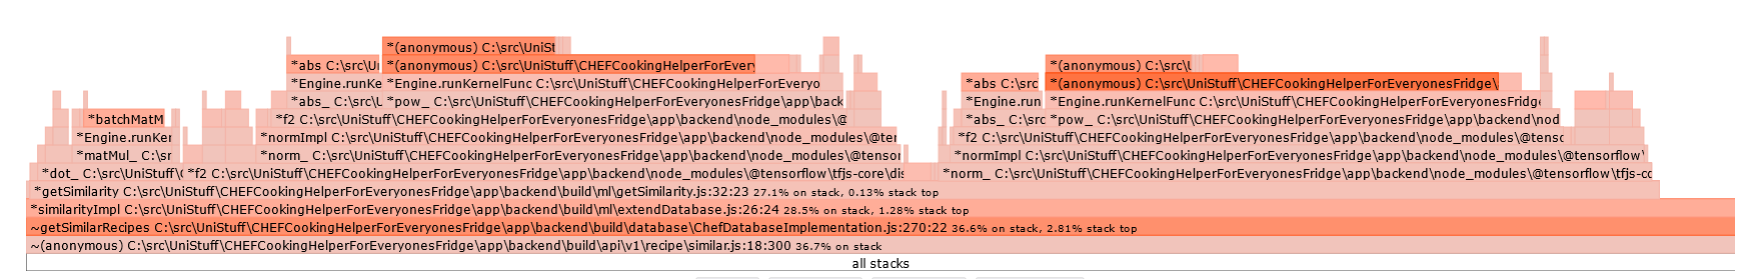
\includegraphics[angle=90,height=0.9\textheight]{figures/similarity_flamegraph.png}
\end{figure}

\begin{figure}
    \centering
    \caption{\label{fig:metalinter_report}A MegaLinter report that was automatically attached as a comment to a pull request.}
    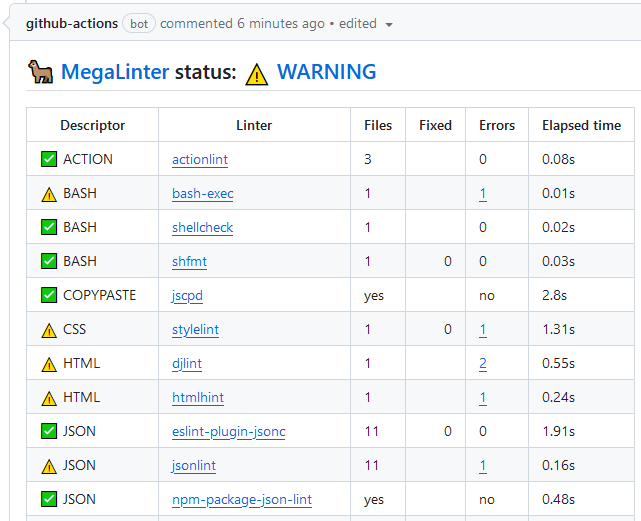
\includegraphics[width=\textwidth]{figures/megalinter_report.png}
\end{figure}

% Appendices


% TODO: Remove todo list once done
\todos{}

%TC:endignore

\end{document}
